\section{The algorithmic agent}

%%%%%%%%%%%%%%%%%%%%%%%%%%%%%%%%%%%%%%%%%%%%%%%%%%
\begin{frame}[label=ladila]{The algorithmic agent}
Minimal set of elements needed for a homeostatic algorithmic system. To be connected with (neuro)biology.
 \begin{center}
  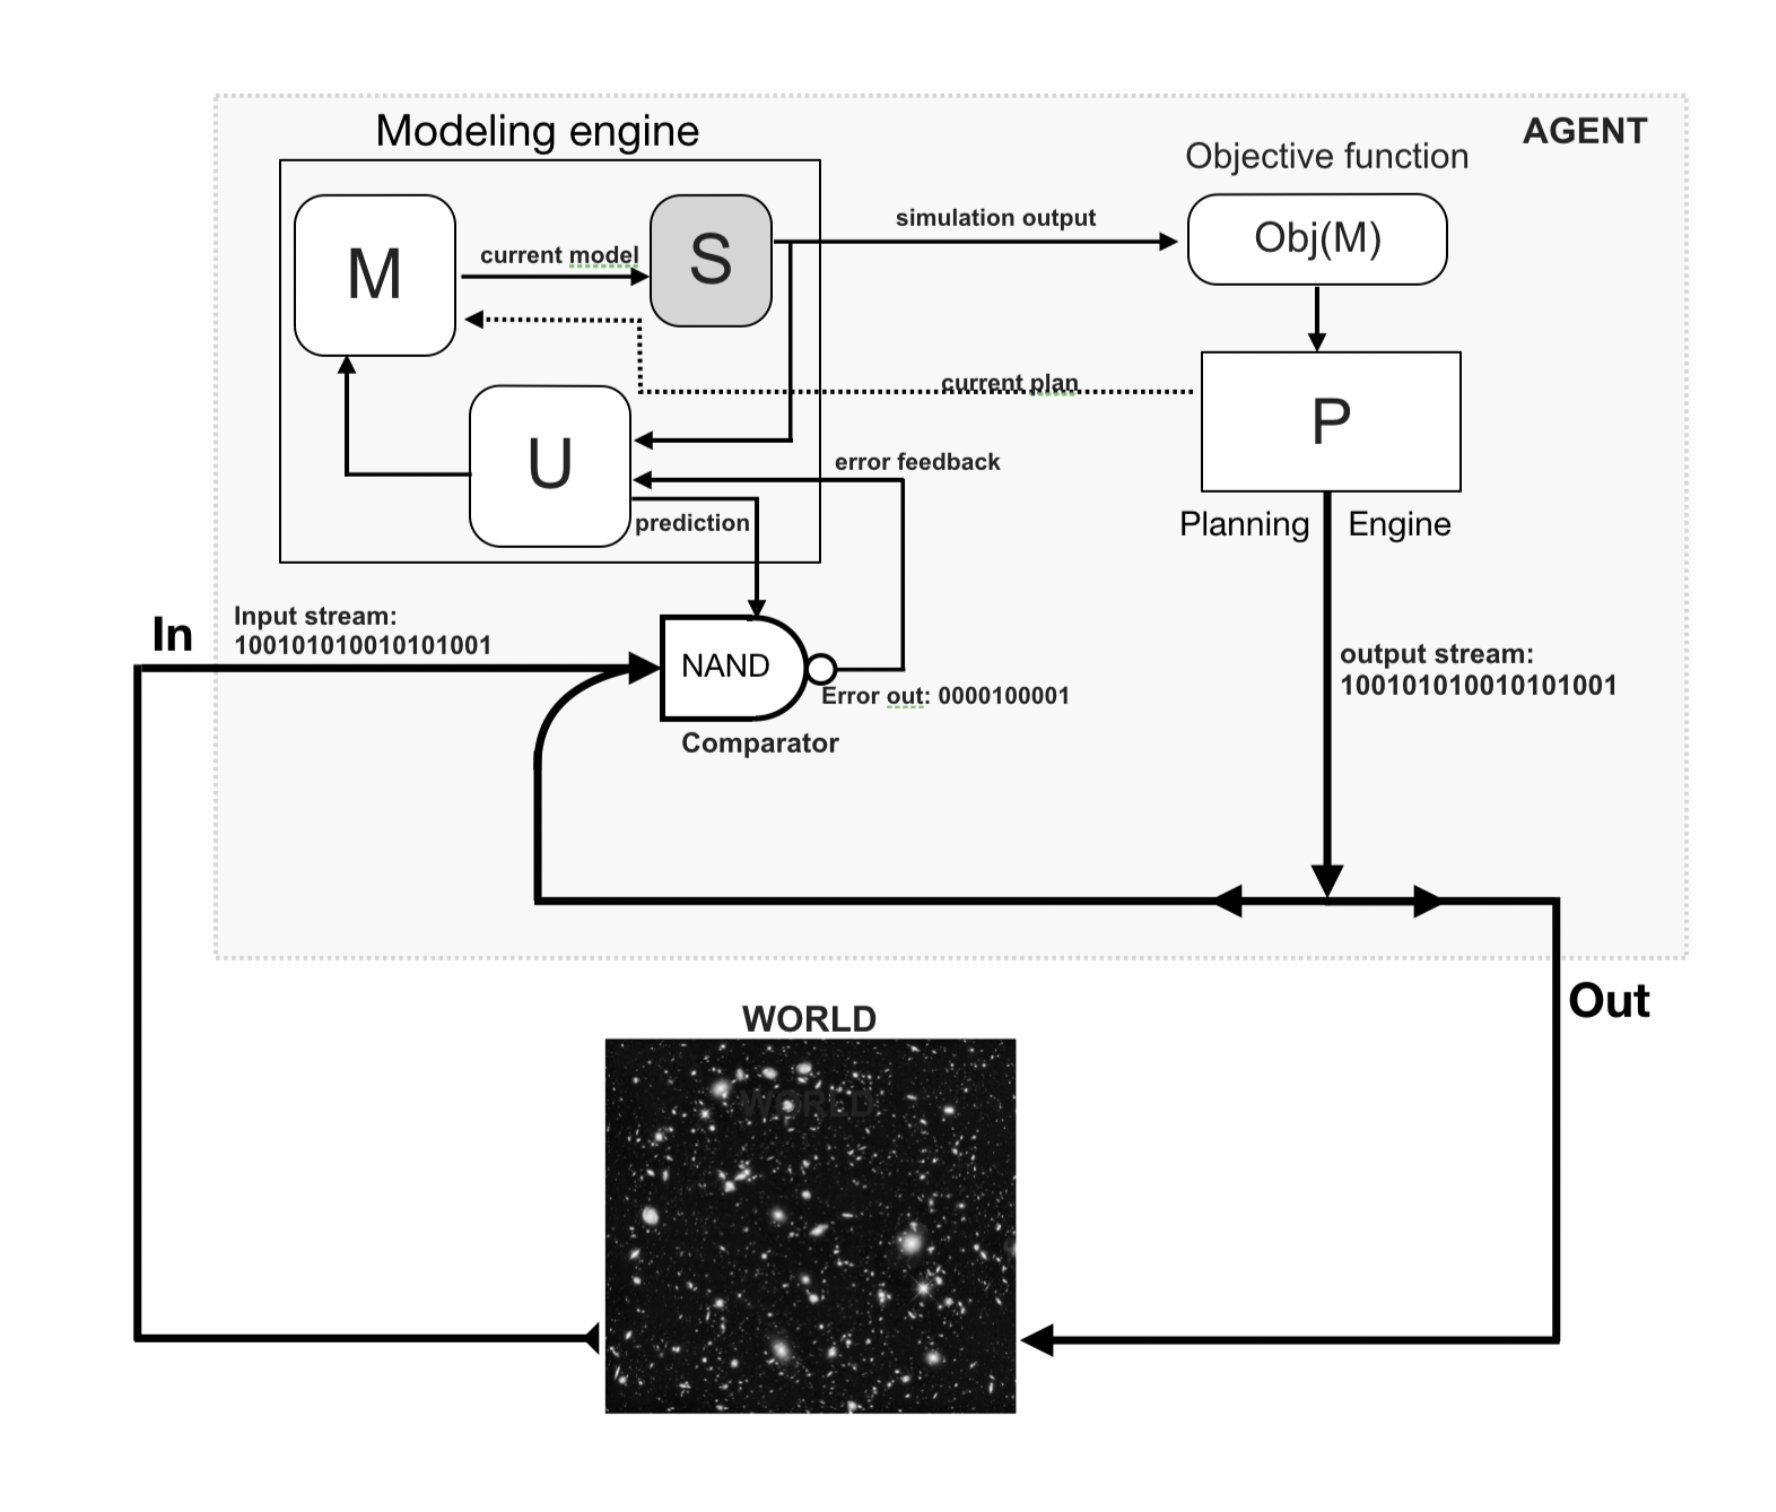
\includegraphics[height=6cm]{img/agent.png}
  \end{center}

\end{frame}



%%%%%%%%%%%%%%%%%%%%%%%%%%%%%%%%%%%%%%%%%%%%%%%%%%
\begin{frame}[label=ladila]{The algorithmic event of \SEP}
Theories of cortical processing emphasize the separation of forward and backward information flow in the cortex also mirrored at the level of single cortical pyramidal cells \citep{CarhartHarris2019,Aru2020}. {\bf Comparator} implemented hierarchically in L5 P cells. \vspace{0.5cm}

 
  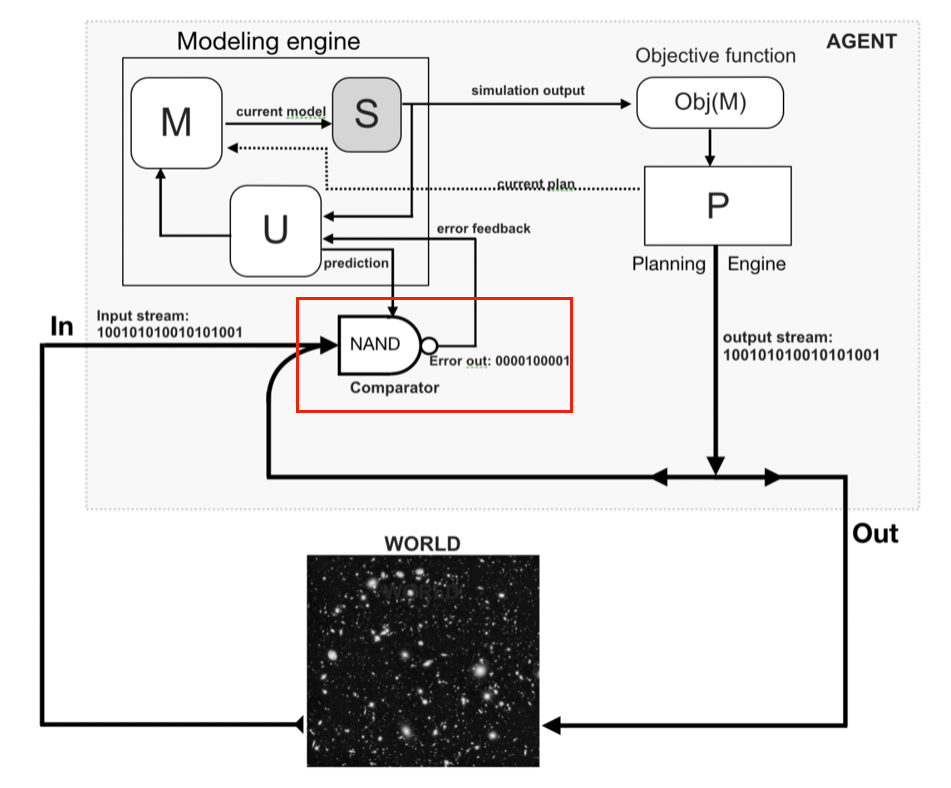
\includegraphics[height=4.cm]{img/agent2.png}
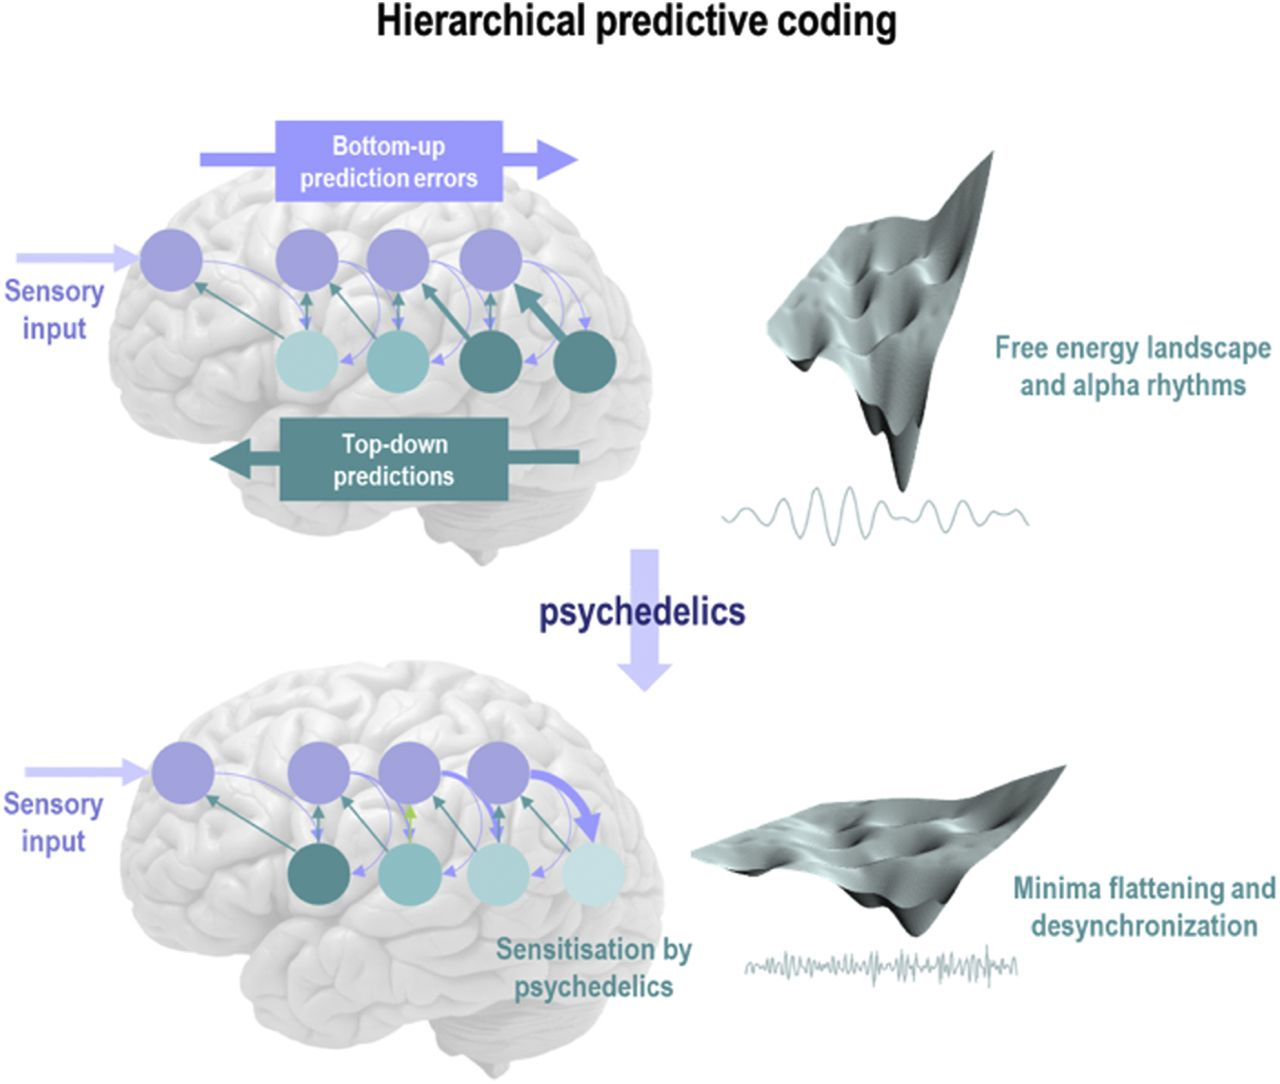
\includegraphics[height=4.cm]{img/F1.large.jpg}
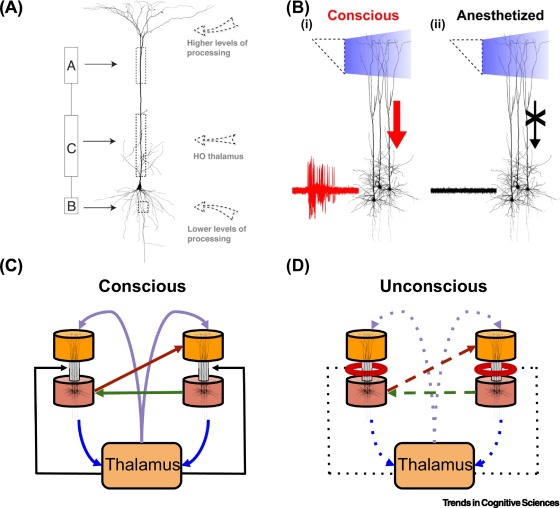
\includegraphics[height=4.cm]{img/gr2.jpeg}
\end{frame}



%%%%%%%%%%%%%%%%%%%%%%%%%%%%%%%%%%%%%%%%%%%%%%%%%%
\begin{frame}[label=ladila]{Model-building I: life}
 How do agents build models? In addressing this, we are led to connecting the concepts of life, intelligence, and \SEP. \vfill
 
 Both life and intelligence represent processes to construct simple models for the persistence of algorithmic information-preserving systems across time. \vfill
 
  Starting from {\em resilient building blocks (static persistence)}, from a computational perspective {\em life} is an algorithmic process: program building carried not solely by the individual agent, but by the transgenerational agent through evolution for {\em meta-homeostasis} (preservation of kind) (v. also \cite{Walker2013, Chaitin2012-wd}).
  
\end{frame}

%%%%%%%%%%%%%%%%%%%%%%%%%%%%%%%%%%%%%%%%%%%%%%%%%%
\begin{frame}[label=ladila]{Model-building II: intelligence}
 Evolutive pressure gives rise to the next leap, {\em intelligence}: agents that, starting from their static model (DNA in life)   build higher-level compressive models of the world within their lifetime, e.g., using brains.\vfill
 
 Importantly, KT holds that both static-model and active-modeling agents enjoy structured experience, only that their level of structure is possibly different.  \vfill
 
 
 [What comes after life and intelligence?]
 
\end{frame}


%%%%%%%%%%%%%%%%%%%%%%%%%%%%%%%%%%%%%%%%%%%%%%%%%%
% \begin{frame}[label=ladila]{Model-building in artificial agents}
% As a consequence of the above, we should explore two routes to the construction of artificial model-building agents: \vfill

% A) {\bf Single generation} model building where agents are endowed with a {\em simplicity bias} (this is what we call the  {\em intelligence} approach). \vfill


% B) {\bf Transgenerational} model building ({\em life}) where the bias for simplicity  emerges naturally from the construction process that favors simple short programs  under evolutionary pressure in {\em  environments governed by simple laws}.  
% \end{frame}